\section{IPC parent-child interactions}
\label{sec:functionality}

We now focus on the interaction between two subnets in a parent-child relation, which is the basic building block of the recursive \ipc hierarchy.
The IPC interface exposes the following functionalities:
\begin{enumerate}

    \item Creating child subnets in the IPC hierarchy.\\
    \emph{E.g., when starting a new game on the gaming platform.}
    
    \item Depositing funds from an account in a subnet to an account in its child.\\
    \emph{E.g., when a player tops up the balance of their account on the gaming platform.}
    
    \item Withdrawing funds from an account in a subnet to an account in its parent.\\
    \emph{E.g., when a player withdraws money they won in a tournament.}
    
    \item Checkpointing a subnet's replicated state in the replicated state of its parent.\\
    \emph{E.g., after every 100 blocks of transactions applied to the gaming platform's subnet.}
    
    \item Invoking actor functions across subnets, i.e., the replicated logic of one subnet acting as a client of another subnet.\\
    \emph{E.g., when a game finishes and its the involved players' rankings are automatically updated.}
    
    \item Removing child subnets from the IPC hierarchy.\\
    \emph{E.g., when a game fihishes, rankings have been updated, and the state of the game can be disposed of.}
    
    \item Managing proof-of-stake subnets, exposing functions for adding and removing replicas, managing the associated collateral, and slashing of provably misbehaving replicas.\\
    \emph{E.g., when mutually distrusting players play together.}
\end{enumerate}
In the following, we describe each functionality in detail, introducing the functions of the \gw and \sa through which this functionality is exposed
and the patterns in which the users and the \ipc agent invoke them via transactions.

\subsection{Creating a child subnet}
\label{sec:create}

To create child subnets, the \gw exposes the following function.
\begin{align*}
    \gw.&\funcName{CreateChild}(\funcParam{subnetName})
\end{align*}
Any user or actor of a subnet \subnetName{P} can create a new child subnet \subnetName{P/C} by
\begin{enumerate}
    \item creating a new instance of the \saFull \saOf{C} and
    \item submitting a transaction \funcNameFull{P}{\gw}{CreateChild}(\subnetName{C}).
\end{enumerate}

The new actor \saOf{C} must configured with all the subnet-specific parameters relevant for governing the new subnet.
These would usually include the used consensus protocol, rules for joining the subnet, definitions and evaluation logic for {\pom}s and {\pof}s, and slashing policies.
From the perspective of the \ipc hierarchy, the subnet is considered created as soon as \saOf{C} is created.
The subnet itself need not necessarily be operational at this moment,
as the parent subnet always has a passive role when it comes to interacting with it.

\begin{example}
\label{ex:create-game-subnet}

Imagine that a player wants to create a game subnet to play against 3 opponents,
such that each player will run their own replica in the game subnet (i.e., their own copy of the game server).
As an incentive for honest behavior, the player decides that the child subnet will be PoS-based (see \Cref{sec:pos-subnets}),
where each replica must be backed by a minimal collateral of 10 coins that would be slashed (and, say, redistributed to the other players) if the replica is caught misbehaving (see \Cref{sec:slash}).

To achieve this, the player creates a subnet actor governing a child subnet that allows replicas to join only if at least 10 of collateral are associated with them
stops accepting new collateral after 4 replicas (the player and 3 opponents) reach the threshold of 10 coins.
The player then registers the new subnet through a \funcNameFull{P}{\gw}{CreateChild} transaction, starts their own replica of the game server (we assume the game server is implemented such that it can be replicated and run as a subnet)
and waits for other players's replicas to join (see \Cref{sec:staking-collateral}).

Note that, since the subnet actor is created by the user, its initial state and logic can be configured arbitrarily.
For example, the \sa could easily be configured with other admission policies (only players with a game ranking within a defined range)
or slashing policies (penalize misbehaving replicas by the backing player loosing not just coins, but also their position in a game-specific ranking system).

\end{example}

\subsection{Depositing funds}
\label{sec:deposit}

A deposit is a transfer of funds from an account in the parent subnet to an account in the child subnet.
The following functions are exposed by the \ipc actors to enable deposits.
\begin{align*}
    \sa.&\funcName{Deposit}(\funcParam{amount, account})\\
    \gw.&\funcName{MintDeposited}(\funcParam{amount, account, \pof})
\end{align*}
The \funcParam{amount} is the amount of funds to be deposited, \funcParam{account} is the destination account in the child subnet, and \funcParam{\pof} is a proof of finality proving that \sa.\funcName{Deposit}(\funcParam{amount, account}) has been applied to the parent subnet's replicated state and that state is final (i.e., cannot be rolled back).

%We assume that the owner of \src is either running their own IPC Agent to perform the necessary operations described below, or uses another trusted IPC agent to act on their behalf.
Depositing \funcParam{amount} coins from an account \accountNameFull{P}{a} in the parent subnet \subnetName{P} to an account \accountNameFull{P/C}{b} in the child subnet \subnetName{P/C}
involves the following steps.

\begin{enumerate}

    \item The owner of \accountNameFull{P}{a} submits, using their wallet, a transaction\\
    \tx{tx} = \funcNameFull{P}{\saOf{C}}{Deposit}(\funcParam{amount}, \accountName{b}).
    
    \item \subnetName{P} orders and executes \tx{tx}, transferring \funcParam{amount} coins from \accountName{a} to \saOf{C}.
    
    \item \label{item:deposit-step-create-pof}
    When \subnetName{P}'s replicated state that includes \tx{tx} becomes final (for some subnet-specific definition of finality provable to \subnetName{P/C}.\gw, which contains the \pof verification logic),
    the \ipc agent constructs a {\pof}(\tx{tx}).
    
    \item \label{item:deposit-step-submit-pof}
    The \ipc agent submits a transaction\\
    \tx{tx'} = \funcNameFull{P/C}{\gw}{MintDeposited}(\funcParam{amount}, \accountName{b}, {\pof}(\tx{tx})).
    
    \item \subnetName{P/C} orders and executes \tx{tx'}, which results in minting \funcParam{amount} new coins and adding them to the balance of \accountNameFull{P/C}{b}.
    
\end{enumerate}

After all the above steps are performed, the newly minted \funcParam{amount} of coins at the child is backed by the analogous locked amount at \subnetName{P}.\saOf{C}.
However, those coins can effectively only be used by the owner of \accountNameFull{P/C}{b},
since \subnetName{P}.\saOf{C} will not transfer its coins within \subnetName{P} until they are burned in \subnetName{P/C} during a withdrawal operation (see below).

\begin{example}
\label{ex:deposit}

Imagine that a player wants to start using the gaming platform (running on the subnet \subnetName{P/C}), but only has funds in an account \accountNameFull{P}{a} in the parent subnet.
To be able to join games that require a collateral (as in \Cref{ex:create-game-subnet}), the player decides to fund their account \accountNameFull{P/C}{b} with 20 coins.
Thus, the player submits a \funcNameFull{P}{\saOf{C}}{Deposit(20, \accountName{b})} transaction, starts an \ipc agent process that performs steps \ref{item:deposit-step-create-pof} and \ref{item:deposit-step-submit-pof} above,
and waits until the funds appear on \accountNameFull{P/C}{b}.

\end{example}

% We show in Algorithm~\ref{alg:deposit} the pseudocode to implement the functionality. 

% \begin{figure}[h]
%      \centering
%      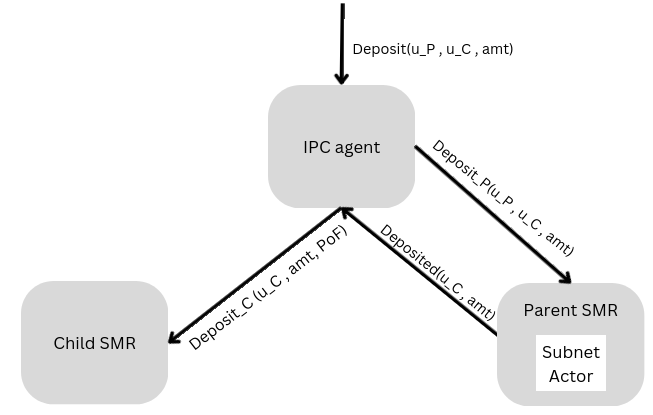
\includegraphics[width=\textwidth]{deposit}
%      \caption{Events produced and consumed during a deposit.}
%      \label{fig:deposit}
% \end{figure}

 
% \begin{algorithm}[H]
% \footnotesize
% \caption{Deposit operation}\label{alg:deposit}
%   \DontPrintSemicolon
%   \SetKwFunction{FMain}{Global}
%   \SetKwProg{Pn}{Function}{:}{\KwRet}
%   \SetKwInOut{Input}{input}
%   \SetKwProg{Component}{$\blacktriangleright$ \bf}{:}{\KwRet}
%   \SetKwFor{UponKW}{upon}{do}{fintq}

%    \Component{Owner of \src}{
%         submit $\tx{tx}=\textit{P.\sa.Deposit}\left( \src, \fil, \dest \right)$ to parent subnet\;
%   }
%    \Component{P.\sa.Deposit(\src, amt, \dest)}{
%     move $\fil$ from \src to P.\sa.\textit{accounts}.\dest  \tcp*[r]{"lock" at parent}
%   }
%   \Component{IPC agent}{
%     \UponKW{tx = P.\sa.Deposit final at parent}{
%         create \prf that \tx{tx} is final at parent subnet \tcp*[r]{see \cref{sec:finality}}
%         submit \textit{P/C.\gw.Deposited(amt, \dest, \pof)}
%      }
%      \jorge{this notation is also a bit weird, in that "upon tx ... final at parent" is running text and it's not immediately obvious that that's the condition}
%   }
%   \Component{P/C.\gw.Deposited(amt, \dest, \pof)}{
% %    \UponKW{\texttt{Deposited}}{
%         verify(\pof)\;
%         increase \dest account by \fil
% %     }
%   }
% \end{algorithm}


\subsection{Withdrawals}
\label{sec:withdraw}

A withdrawal is a transfer of funds from an account in the child subnet to an account in the parent subnet.
The following functions are exposed by the \ipc actors to enable withdrawals.
\begin{align*}
    \gw.&\funcName{Withdraw}(\funcParam{amount, account})\\
    \sa.&\funcName{ReleaseWithdrawn}(\funcParam{amount, account, \pof})
\end{align*}
The \funcParam{amount} is the amount of funds to be withdrawn, \funcParam{account} is the destination account in the parent subnet to which the withdrawn funds are to be credited, and \funcParam{\pof} is a proof of finality proving that \gw.\funcName{Withdraw}(\funcParam{amount, account}) has been applied to the child subnet's replicated state and that state is final (i.e., cannot be rolled back).

Withdrawing \funcParam{amount} coins from an account \accountNameFull{P/C}{b} in the child subnet \subnetName{P/C} to an account \accountNameFull{P}{a} in the parent subnet \subnetName{P}
involves the following steps.

\begin{enumerate}

    \item The owner of \accountNameFull{P/C}{b} submits, using their wallet, a transaction\\
    \tx{tx} = \funcNameFull{P/C}{\gw}{Withdraw}(\funcParam{amount}, \accountName{a}).
    
    \item \subnetName{P/C} orders and executes \tx{tx}, burning \funcParam{amount} coins from \accountName{b}.%
    
    \item When \subnetName{P/C}'s replicated state that includes \tx{tx} becomes final (for some subnet-specific definition of finality provable to \subnetName{P}.\saOf{C}),
    The \ipc agent constructs a {\pof}(\tx{tx}).
    
    \item The \ipc agent submits a transaction%
    \footnote{In a practical implementation, instead of submitting a separate transaction for each withdrawal,
    the \ipc agent may submit multiple withdrawals batched in a single transaction,
    with a single \pof proving the finality of the child state in which all the corresponding funds have been burned.
    This optimizes both performance and cost (transaction fees) at the parent.
    Our implementation applies this optimization, further combined with checkpoints.}\\
    \tx{tx'} = \funcNameFull{P}{\saOf{C}}{ReleaseWithdrawn}(\funcParam{amount}, \accountName{a}, {\pof}(\tx{tx})).
    
    \item \subnetName{P} orders and executes \tx{tx'}, which results in \subnetName{P}.\saOf{C} transferring \funcParam{amount} coins to account \accountNameFull{P}{a}.
    
\end{enumerate}

The above procedure ensures that the locked \funcParam{amount} at the parent is not released until the child has already burned the minted \funcParam{amount} of coins.
The \subnetName{P}.\saOf{C} actor ensures (by verifying the associated \pof) that the coins have been burned in \subnetName{P/C}
before releasing the corresponding \funcParam{amount} back into circulation in \subnetName{P}.

\begin{example}
\label{ex:withdrawal}
A player might want to stop using the gaming platform and withdraw all the funds back to the parent subnet, in order to spend them on something else.
They still have 20 coins on their account \accountNameFull{P/C}{b} that they want to transfer back to \accountNameFull{P}{a}.
The player performs the withdrawal by submitting a transaction \funcNameFull{P/C}{\gw}{Withdraw(20, \accountName{a})},
starts an \ipc agent process to perform the necessary inter-subnet communication, and waits until the coins arrive at \accountNameFull{P}{a}.
(The player might need to spend a part of the 20 coins on fees for both the \funcName{Withdraw} and the \funcName{ReleaseWithdrawn} transactions.)
\end{example}

% OLD VERSION
% A withdrawal is a transfer of funds from an account \src in the child subnet $P/C$ to an account \dest in the parent subnet $P$.
% The \emph{Withdraw} is performed analogously to the \emph{Deposit}, but starting at the child subnet $P/C$:
% \begin{enumerate}
%   \item The owner of \src submits a transaction \emph{tx =} $\textit{P/C.\gw.Withdraw}(\src, \fil, \dest)$.
%     \item The child subnet orders and executes the \emph{Withdraw} transaction, burning $\fil$ funds in $\src$ (provided $\src$ has enough funds).
%     \item When the child's replicated state that includes the transaction becomes final (for some SMR-system-specific definition of finality that has been defined in the SA), the \ipc agent constructs a corresponding \pof and submits a transaction \textit{\tx{tx'} = P.\sa.Withdrawn(\fil, \dest, \pof)} to the parent subnet.
%     \item Upon ordering $\tx{tx'}$, \emph{P.\sa.Withdrawn(amt, \dest, \pof)} verifies the \pof and transfers \emph{amt} from \sa (concretely, to $\src$ account representation within the \sa) to $\dest$ within the parent subnet.
% \end{enumerate}

%  % \begin{figure}[h]
%  %     \centering
%  %     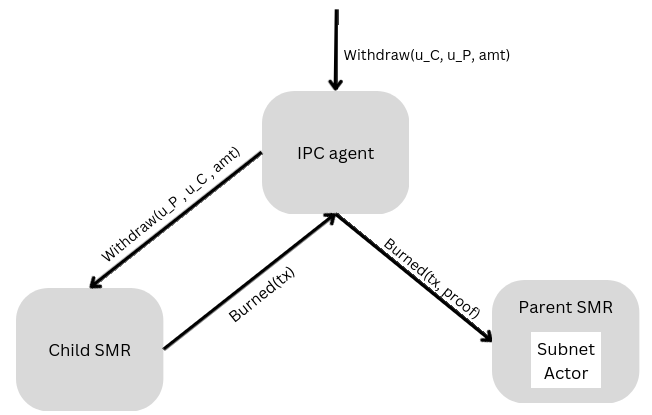
\includegraphics[width=\textwidth]{withdrawal}
%  %     \caption{Events produced and consumed during a withdrawal.}
%  %     \label{fig:withdrawal}
%  % \end{figure}
%  We show in Algorithm~\ref{alg:withdraw} the pseudocode to implement the functionality. 

% \begin{algorithm}[H]
% \footnotesize
% \caption{Withdraw operation}\label{alg:withdraw}
%   \DontPrintSemicolon
%   \SetKwFunction{FMain}{Global}
%   \SetKwProg{Pn}{Function}{:}{\KwRet}
%   \SetKwInOut{Input}{input}
%   \SetKwProg{Component}{$\blacktriangleright$ \bf}{:}{\KwRet}
%   \SetKwFor{UponKW}{upon}{do}{fintq}
%   % \Input{user~$\user$, amount~$\fil$, transaction \txnf}
%    \Component{owner of \src}{
%         submit $\tx{tx}=\textit{P/C.\gw.Withdraw}(\src, \fil, \dest)$\;
%   }
%    %
%    \Component{\textit{P/C.\gw.Withdraw(\src, \fil, \dest)}}{
%     deduct $\fil$ from \src \tcp{"burns" \fil in child}
%   }
%   \Component{IPC agent}{
%     \UponKW{tx = P/C.\gw.Withdraw(\src, \fil, \dest) final at child}{
%         create $\pof(tx)$ \tcp*[r]{see \cref{sec:finality} for details}
%         submit \textit{P.\sa.Withdrawn(amt, \dest, \pof)}
%      }
%   }
%   \Component{P.\sa.Withdrawn(amt, \dest, \pof)}{
%     verify($\pof(tx')$)\;
%     move \fil coins from P.\sa to \dest \tcp{"unlocks" \textit{amt} for \dest}
%   }
   
% \end{algorithm}
% \label{enhancedFunc}

\subsection{Checkpointing} 
Checkpointing is a method for a parent subnet to keep a record of the evolution of its child subnet's replicated state
by including snapshots of the child's replicated state (called checkpoints) in the parent's replicated state.
If, for some reason, the child subnet misbehaves as a whole (e.g., by a majority of its replicas being taken over by an adversary), 
agreement can be reached in the parent subnet about how to proceed.
For example, which checkpoint should be considered the last valid one.
The following function is exposed by the \sa to enable checkpointing.

\begin{align*}
    \sa.&\funcName{Checkpoint}(\funcParam{snapshot}, \pof)
\end{align*}

A checkpoint can be triggered by predefined events (e.g.,  periodically, after a number of state updates, triggered by a specific user or set of users, etc.).
The \ipc agent is configured with the (subnet-specific) checkpoint trigger, monitors the child subnet's replicated state,
and takes the appropriate action when the trigger condition is satisfied by the child subnet's state.
A checkpoint of subnet \subnetName{P/C} to its parent \subnetName{P} is created as follows:
\begin{enumerate}

    \item When the predefined checkpoint trigger is met in the replicated state of \subnetName{P/C},
    the \ipc agent retrieves the corresponding snapshot of \subnetName{P/C}'s replicated state (\emph{state}) from the child subnet, along with the proof of its finality {\pof}(\emph{state}).

    \item The \ipc agent submits a transaction\\
    \tx{tx} = \funcNameFull{P}{\saOf{C}}{Checkpoint}(\funcParam{state}, {\pof}(\funcParam{state})).

    \item \subnetName{P} orders and executes \tx{tx}, which results in \subnetName{P}.\saOf{C} including \funcParam{state}
    (i.e., the checkpoint of \subnetName{P/C}'s replicated state) in its own actor state.

\end{enumerate}

% \TODO{Pseudocode}
% See commented algorithm

% \begin{figure}[h]
%      \centering
%      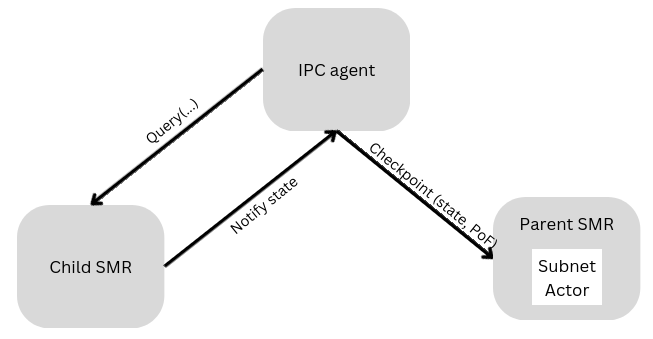
\includegraphics[width=\textwidth]{checkpoint.png}
%      \caption{Events produced and consumed by the checkpointing functionality.}
%      \label{fig:chkp}
%  \end{figure}
% \del{
% Note that we do not show here incentives for participants to submit checkpoints, the same way we do not discuss in Algorithm~\ref{alg:checkpoint} whether the particular participant running the IPC agent has even rights to submit the checkpoint. We show instead in Section~\ref{sec:incentives} different mechanisms that can be used to incentivize participants running IPC agents, while in Section~\ref{sec:ref-impl} we describe how the reference implementation of IPC incentivizes and gives participants the right to submitting checkpoints. Analogously, we discuss in Section~\ref{sec:ref-impl} optimizations and other design decisions made to the checkpoint operation.
% }


% \begin{algorithm}[H]
% \footnotesize
% \caption{Checkpoint operation}\label{alg:checkpoint}
%   \DontPrintSemicolon
%   \SetKwFunction{FMain}{Global}
%   \SetKwProg{Pn}{Function}{:}{\KwRet}
%   \SetKwInOut{Input}{input}
%   \SetKwProg{Component}{$\blacktriangleright$ \bf}{:}{\KwRet}
%   \SetKwFor{UponKW}{upon}{do}{fintq}

%   \Component{IPC agent}{
%     \UponKW{Checkpoint condition in child}{
%       $chkp = $ obtain state snapshot from child\;
%       create $\pof(chkp)$\;
%       submit $P.\sa.Checkpoint(chkp, \pof(chkp))$
%     }
%   }

%   \Component{P.\sa.Checkpoint(chkp, \pof(chkp))}{
%     verify($\pof(tx')$)\;
%     save $chkp$ in the state\;
%     % \TODO{Expand on this. check if the checkpoint is the latest one and use a variable to store the latest checkpoint}
%   }
   
% \end{algorithm}

% OLD PSEUDOCODE
% \begin{algorithm}[H]
% \footnotesize
% \caption{Checkpoint operation\TODO{Update to new terminology}}\label{alg:down}
%   \DontPrintSemicolon
%   \SetKwFunction{FMain}{Global}
%   \SetKwProg{Pn}{Function}{:}{\KwRet}
%   \SetKwInOut{Input}{input}
%   \SetKwProg{Component}{$\blacktriangleright$ \bf}{:}{\KwRet}
%   \SetKwFor{UponKW}{upon}{do}{fintq}
%    \Component{IPC agent}{
%         \If{trigger for checkpoint}{
%             \textit{SA\_state} $\gets$ query parent for \sa's state\;
%             \If{\textit{Self} \textbf{in} SA\_state.validators}{
%                 \textit{state} $\gets$ query child for state\;
%                 \textit{cState} $\gets$ \textit{compressState}(\text{state},\textit{SA\_state.latestCheckpoint})\;
%                 create \prf that \textit{cState} is final at child\;
%             }
%             $\tx{tx}=\sa.\texttt{Checkpoint}\left(\textit{cState}, \prf \right)$ \;
%             \If{\textit{Self.}\ssc(tx, SA\_state, ...)}{
%                 submit $tx$ to parent \smr replica\;
%             }
%         }
%   }
%   \Component{parent \smr replica}{
%     \UponKW{$\tx{tx}=\sa.\texttt{Checkpoint}\left(\textit{cState}, \prf \right)$}{
%         assert \sa.\verifyGfinal{\textit{cState}}{\prf}\;
%         $\sa.\textit{latestCheckpoint.update}(\textit{cState})$
%      }
%   }
% \end{algorithm}

% The above pseudo code is intentionally abstract, with a number of implementation decisions not specified, such as the main function for creating and verifying a \prf, events that trigger the creation of a new checkpoint, the compression procedure with respect to the previous checkpoint, and the \ssc function to decide whether the participant submits or not a checkpoint. 

% The above pseudo code is highly abstract, with the main function of creating and verifying a \prf not specified. Moreover, other important aspects that are not covered include specific compression mechanisms for the checkpoint data, triggering checkpoints efficiently, and particular incentives for checkpoints creation and submission. \arp{we refer to reference implementation... later in this document we list others...}
% The function \ssc comprises two aspects of the checkpointing functionality from the perspective of participants. First, it controls access to submit checkpoints, as not all subnets will define the same policy to follow when deciding the participants that are allowed to submit checkpoints. Second, it contains the implications of submitting a checkpoint transaction (i.e. the cost involved in being the submitter). For example, if only one transaction is required by any participant but the cost of submitting the checkpoint is incurred on the submitter, then there is a risk of no participant actually submitting the checkpoint if they are strictly rational. An example on the other end might be requiring all participants to submit a transaction for the checkpoint to be finalized at the parent, but this approach affects performance. \arp{We analyze and suggest later in this document multiple mechanisms to ensure through incentives that at least one rational participant will always submit the checkpoint. }

\subsection{Propagating cross-net transactions}
\label{sec:cross-net-tx}

Cross-net transactions are a means of interaction between actors located on different subnets.
Unlike a "standard" transaction issued and submitted to a subnet by a user's wallet,
a cross-net transaction is issued by actors of another subnet.

Since those actors themselves are not processes (but mere parts of a subnet's replicated state),
they cannot directly submit transactions to other subnets.
IPC therefore provides a mechanism to propagate these transactions between subnets using the following functions of the \gw.

\begin{align*}
    \gw.&\funcName{Dispatch}(\funcParam{tx, src, dest})\\
    \gw.&\funcName{Propagate}(\funcParam{tx, src, dest, \pof})
\end{align*}

In a nutshell, if an actor's logic in subnet $\subnetName{S}_1$ produces a transaction for a different subnet $\subnetName{S}_2$,
it calls $\subnetName{S}_1$.\gw.\funcName{Dispatch}, which saves the transaction in $\subnetName{S}_1$'s \gw buffer that we call the \postoffice.
IPC agents, monitoring the \postoffice, then iteratively submit the transaction to the appropriate next subnet along the path from $\subnetName{S}_1$ to $\subnetName{S}_2$ using \gw.\funcName{Propagate}.

Since, in general, we only rely on IPC Agents to be able to submit transactions to parents or children of a subnet whose state they observe,
an IPC agent only propagates the transaction to the parent or child, depending on which is next along the shortest path from $\subnetName{S}_1$ to $\subnetName{S}_2$ in the IPC hierarchy.
After such ``one hop``, the transaction is again placed in the \postoffice of the parent / child, and the process repeats until the transaction reaches its destination subnet.

More concretely, we illustrate the propagation of a cross-net transaction using an example where an actor in subnet \subnetName{P/A}
is sending a cross-net transaction \tx{tx} to its "sibling" subnet \subnetName{P/B}.
\tx{tx} is first propagated from \subnetName{P/A} to its parent \subnetName{P}, which, in turn, propagates it to its other child \subnetName{P/B}.
We use the function \gw.\funcName{Dispatch} in a subnet to announce that the transaction is ready to be propagated
and the function \gw.\funcName{Propagate} to notify a subnet about a cross-net transaction to be passed on (or delivered, if the destination has been reached).

\begin{enumerate}

    \item An actor \subnetName{P/A}.\actorName{ActorA} constructs a tarnsaction\\
    \tx{tx} = \funcNameFull{P/B}{ActorB}{SomeFunction}(\funcParam{someParams})

    \item \subnetName{P/A}.\actorName{ActorA} invokes the funcion \funcNameFull{P/A}{\gw}{Dispatch}(\tx{tx}, \subnetName{P/A}, \subnetName{P/B})
    (note that no additional transactions are necessary here).

    \item The implementation of \funcNameFull{P/A}{\gw}{Dispatch} adds \tx{tx} along with the routing metadata to a local collection-type data structure
    that we call \postoffice and denote \subnetName{P/A}.\gw.\dataField{\postoffice}.

    \item \label{item:first-propagation} Let $state_\subnetName{A}$ be the state of subnet \subnetName{P/A} where \tx{tx} is already included in \subnetName{P/A}.\gw.\dataField{\postoffice}.
    When the \ipc agent responsible for the interaction between \subnetName{P/A} and \subnetName{P} detects that $state_\subnetName{A}$ is final,
    it constructs a {\pof}($state_\subnetName{A}$) and submits a transaction\\
    $\tx{tx}_\subnetName{A}$ = \funcNameFull{P}{\gw}{Propagate}(\tx{tx}, \subnetName{P/A}, \subnetName{P/B}, {\pof}($state_\subnetName{A}$)).

    \item Subnet \subnetName{P} orders and executes $\tx{tx}_\subnetName{A}$, verifying {\pof}($state_\subnetName{A}$)
    and (internally) invoking \funcNameFull{P}{\gw}{Dispatch}(\tx{tx}, \subnetName{P/A}, \subnetName{P/B}).
    This, in turn, adds \tx{tx} along with its routing metadata to \subnetName{P}'s \postoffice \subnetName{P}.\gw.\dataField{\postoffice}.

    \item Analogously to step \ref{item:first-propagation}, the \ipc agent submits a transaction\\
    $\tx{tx}_\subnetName{P}$ = \funcNameFull{P/B}{\gw}{Propagate}(\tx{tx}, \subnetName{P/A}, \subnetName{P/B}, {\pof}($state_\subnetName{P}$)),
    where $state_\subnetName{P}$ is the state of \subnetName{P} with \tx{tx} already included in \subnetName{P}.\gw.\dataField{\postoffice}.

    \item Upon ordering and executing $\tx{tx}_\subnetName{P}$, \funcNameFull{P/B}{\gw}{Propagate} verifies {\pof}($state_\subnetName{P}$).
    Detecting that the destination is the own subnet, the implementation of \funcNameFull{P/B}{\gw}{Propagate} executes \tx{tx} instead of propagating it.

\end{enumerate}

\begin{example}

In our gaming example, imagine that a game (running in its own subnet that is a child of the gaming platform's subnet) has finished and the ranking of the involved players needs to be updated.
The game server is implemented as an actor on the game's own subnet, while the gaming platform (storing the player ranking tables) is an actor of its parent.
To update the ranking, the game actor would use a cross-net transaction to inform the platform actor about the results of the game and the platform actor would update the rankings accordingly.

\end{example}

% The implementation of the \gw's \emph{Propagate} function is sketched in \Cref{alg:po}.

% \TODO{Outline algorithm in text, like in the rest of functionalities.}

% % \guy{Edge case: a leaf subnet does not have a \sa and, therefore, no \postoffice. We can consider removing the \postoffice functionality from the \sa and to deploy it as an independent \actor that will appear only once per subnet. In this case, it needs permissions to call \sa.\verifyGfinal{\tx{tx}}{\prf} function.}

% \begin{algorithm}[H]
% \footnotesize
% \caption{Cross-net transaction propagation functionality}\label{alg:po}
%   \DontPrintSemicolon
%   \SetKwFunction{FPropagate}{propagate}
%   \SetKwProg{Pn}{Function}{:}{\KwRet}
%   \SetKwInOut{Input}{input}
%   \SetKwProg{Component}{$\blacktriangleright$ \bf}{:}{\KwRet}
%   \SetKwProg{Empty}{\bf}{:}{\KwRet}
%   \SetKwFor{UponKW}{upon}{do}{fintq}
%   \Component{\add{S.}\gw.Propagate($\tx{tx}, \src, \dest, \pof)$)}{
%     verify(\tx{tx}.\pof)\;
%     \Case{\dest = \src}{
%         apply \tx{tx}
%     }
%     \Case{\dest requires going up the tree}{
%        $\postoffice \leftarrow \postoffice \cup (\tx{tx}, \replace{S/\src}{src.Parent}, \dest)$\;
%     }
%     \Case{\dest requires going down the tree \add{to child $S_c$}}{
%         $\postoffice \leftarrow \postoffice \cup (\tx{tx}, \replace{\src/S}{S_c}, \dest)$\;
%     }
%   }
%   \Component{IPC agent}{
%     \UponKW{new entry (\tx{tx}, \src, \dest) in \replace{parent}{S}.\gw.\postoffice}{
%         Create \pof proving that \tx{tx'} has indeed been added to the list of cross-net transactions in the subnet\;
%         submit \tx{tx'}, augmented by \emph{\pof}
%     }   
%     % \jorge{do we need to discuss the matter of implicit execution (or future multisig protocol)? maybe a question for Alfonso}\arp{not here imo (this is not the reference implementation), we discuss it in section \ref\{sec:ref-impl}}
% }
% \end{algorithm}

\subsection{Removing a child subnet}
\label{sec:remove}

TODO
% A child subnet $P/C$ can be removed from its parent $P$ through a transaction invoking $P.\gw.RemoveChild(P/C)$. \add{This transaction effectively deregisters the subnet from the IPC hierarchy. We detail further how to remove a child subnet for the reference implementation in~\cref{sec:ref-impl}.}

\subsection{Proof-of-stake subnets}
\label{sec:pos-subnets}

% \arp{I do not think we should particularize in PoS subnets. We just require a wrapper of any blockchain into single finality (with assumption on PoF for PoW-style blockchains after x amount of blocks). For example, for non-PoS children, the IPC agent can require joining and leaving as replica in order for a withdrawal/cross-net/checkpoint from a replica to be valid (even at the child itself, if replica in PoW child subnet creates block but replica not part of membership according to \sa, block is rendered invalid). Slashing can be performed on PoW replicas this way as well (i.e. time-lock withdrawals/release of funds $+$ synchrony). So these operations are not really PoS-specific. The only thing that is not immediately if not PoS is a direct mapping between voting rights (amount of work in PoW) and collateralized amount (this can be solvable limiting amount transferred in blocks for added security, or other measures, for example), but besides it being technically possible, it is also kind of ok since the collateral in PoW is anyways the cost to produce blocks.}
% \matej{I agree that, technically, some of the concepts around collateral and slashing could be, in some way, applied to non-PoS subnets,
% even though I'd argue that it'd be quite a stretch in practice in my opinion.
% Unless you strongly oppose calling this PoS features, I'd suggest staying with the current approach, mostly for time reasons,
% and we can refine / generalize later when we have other critical things sorted out.
% Especially since we do say that the staked collateral determines the voting power, I think it's completely fair to call it PoS.}\arp{Time shortage is a valid reason, but note that we do not require that collateral determines voting power (we do not even conceptually require a minimum amount of collateral at the parent for the child to run its consensus protocol, same way we do not require any specific slashing rule), which adds to the mnuch simpler requirement of single finality (or capped finalization with asumption of single finality, like in Filecoin as rootnet). Let us leave it like this for now and modify later if reused with more time} 

In order to disincentivize replicas of a subnet from misbehaving, \ipc provides a mechanism for conditioning a replica's participation in the child subnet on \emph{collateral} in a proof-of-stake fashion.
To this end, the \sa can associate each replica of the child subnet with a collateral.
Replicas must transfer this collateral to the \sa, and the \sa only releases the collateral back once the corresponding replica stops participating in the subnet. The way in which the collateral associated with replicas impacts the functioning of the child is subnet-specific.

If a child replica provably misbehaves, the proof of such misbehavior can be submitted as a transaction to the \sa (invoking its \emph{Slash} function).
The \sa then decreases the amount of collateral associated with the offending replica in accordance with its (subnet-specific) slashing policy.

Note that collateral is different from funds deposited for use in the child subnet.
Unlike the deposited funds, collateral is not made available in the child subnet
and stays in the parent's \sa until the associated replica stops participating in the subnet, either by leaving or by being slashed.

The advantage of this approach is that a child subnet can leverage funds in the parent subnet to serve as collateral.
In case of provable misbehavior even of replicas that have gained complete power over the child subnet (e.g., by having staked most of the collateral),
those replicas can still be slashed at the parent.
It also prevents long-range \cite{} and similar attacks by maintaining membership information (sometimes also referred to as power table) of the child subnet at the parent.
The membership saved in the \sa's state defines the ground truth about what replicas the child subnet should consist of,
as well as their relative voting power (proportional to the staked collateral) in the underlying ordering protocol.
The child subnet observes the state of the \sa in the parent and, when the membership information changes, reconfigures accordingly.

Since we expect PoS-based child subnets to become very common,
\ipc provides the following native functionality for managing PoS-based subnets:
\begin{itemize}
    \item Manipulate the membership by staking and releasing collateral associated with replicas
    \item Slashing, where \ipc permanently removes / redistributes a part of the collateral associated with a provably misbehaving replica (e.g., one that sends conflicting messages in the ordering protocol)
\end{itemize}

\Cref{ex:create-game-subnet} provides a concrete case of where and how PoS-based subnets can be used.

\subsubsection{Staking collateral}
\label{sec:staking-collateral}

To increase a replica's collateral in a PoS-based subnet, \ipc uses the following functions.

\begin{align*}
    \sa.&\actorName{StakeCollateral}(\funcParam{account, replica, amount})\\
    \gw.&\actorName{UpdateMembership}(\funcParam{membership, \pof})
\end{align*}

Concretely, to increase the amount of collateral associated with a \funcParam{replica} in subnet \subnetName{P/C},
collateral must be staked for \funcParam{replica} in the parent \subnetName{P}'s \saFull \subnetName{P}.\saOf{C}.
Let the the account from which the collateral is transfered to \subnetName{P}.\saOf{C} be \accountNameFull{P}{a}.
(Any user with sufficient account balance (at least \funcParam{amount}) can perform this operation.)

The child subnet, holding its own local copy of the target membership, is then informed (through an \ipc agent) about the membership change and reconfigures to reflect it.
Note that it is required for the child subnet to hold a copy of the membership in its replicated state, so that all its replicas observe it in a consistent way.
In fact, the child subnet replicated state contains two versions of membership information:
\begin{itemize}
    \item The \emph{target membership}, which is a local copy of the membership stored in \subnetName{P}.\saOf{C} and designates the desired membership of the child subnet
    to which the subnet must reconfigure.
    \item The \emph{current membership}, which is the actual membership currently being used by the subnet to order and execute transactions.
    Since the process of reconfiguration to a new membership is usually not immediate, the current membership may "lag behind" the target membership.
\end{itemize}
The whole staking procedure is as follows.

\begin{enumerate}

    \item The owner of \accountNameFull{P}{a} submits the transaction\\
    \tx{tx} = \funcNameFull{P}{\saOf{C}}{StakeCollateral}(\accountNameFull{P}{a}, \funcParam{replica}, \funcParam{amount}).

    \item After ordering \tx{tx}, \subnetName{P}.\saOf{C} increases the collateral associated with \funcParam{replica} by \funcParam{amount},
    which is deducted from the submitting user's account in \subnetName{P}.
    If no collateral has been previously associated with \funcParam{replica}, this effectively translates in \funcParam{replica} joining the subnet.

    \item \label{item:update-membership} The \ipc agent, upon detecting the updated \funcParam{membership} in \subnetName{P}.\saOf{C} through the application of \tx{tx},
    constructs a {\pof}(\tx{tx}) and submits the transaction\\
    \tx{tx'} = \funcNameFull{P/C}{\gw}{UpdateMembership}(\funcParam{membership}, {\pof}(\tx{tx})).

    \item Upon ordering \tx{tx'} and successfully verifying {\pof}(\tx{tx}), \subnetName{P/C}.\gw updates its target membership.

    \item Subnet \subnetName{P/C} reconfigures (the reconfiguration procedure is specific to the implementation of the subnet and its ordering protocol)
    to use the new \funcParam{membership} as its current membership.
    
\end{enumerate}

\subsubsection{Releasing collateral}

Releasing collateral works similarly (but inversely) to staking, with one significant difference.
Namely, once the child subnet \subnetName{P/C} reconfigures to reflect the updated membership, the parent's \saFull \subnetName{P}.\saOf{C} does not release the staked funds
until it is given a proof that the child subnet \subnetName{P/C} finished the (subnet-specific) reconfiguration procedure
and that no replica has more voting power than corresponds to its collateral after the release.
The following functions are involved in releasing collateral:

\begin{align*}
    \sa.&\actorName{RequestCollateral}(\funcParam{replica, amount, account})\\
    \gw.&\actorName{UpdateMembership}(\funcParam{membership, \pof})\\
    \sa.&\actorName{ReleaseCollateral}(\funcParam{membership, \pof})
\end{align*}

Let \accountNameFull{P}{a} be an account that has staked collateral for a \funcParam{replica} in a PoS-based subnet \subnetName{P/C}.
The procedure for releasing collateral is as follows.

\begin{enumerate}

    \item The owner of \accountNameFull{P}{a} submits the transaction\\
    \tx{tx} = \funcNameFull{P}{\saOf{C}}{RequestCollateral}(\funcParam{replica}, \funcParam{amount}, \accountName{a}),\\
    where \funcParam{amount} is the amount of funds the owner of \accountNameFull{P}{a} wants to reclaim.

    \item After ordering \tx{tx} and checking that \accountNameFull{P}{a} has indeed previously staked at least \funcParam{amount} for \funcParam{replica},
    \subnetName{P}.\saOf{C} decreases the collateral associated with \funcParam{replica} by \funcParam{amount}.
    Note that \subnetName{P}.\sa does not yet transfer \funcParam{amount} back to \accountNameFull{P}{a}

    \item The \ipc agent, upon detecting the updated \funcParam{membership} in \subnetName{P}.\saOf{C} through the application of \tx{tx},
    constructs a {\pof}(\tx{tx}) and submits the transaction\\
    \tx{tx'} = \funcNameFull{P/C}{\gw}{UpdateMembership}(\funcParam{membership}, {\pof}(\tx{tx})).

    \item Upon ordering \tx{tx'} and successfully verifying {\pof}(\tx{tx}), \subnetName{P/C}.\gw updates its target membership.

    \item Subnet \subnetName{P/C} reconfigures (the reconfiguration procedure is specific to the implementation of the subnet and its ordering protocol)
    to use the new \funcParam{membership} as its current membership.

    \item The \ipc agent detects that the current membership of \subnetName{P/C} has changed.
    Let \funcParam{state} be the the replicated state of \subnetName{P/C} where the current membership has already been updated.

    \item The \ipc agent constructs a {\pof}(\funcParam{state}) and submits the transaction\\
    \tx{tx''} = \funcNameFull{P}{\saOf{C}}{ReleaseCollateral}(\funcParam{membership}, {\pof}(\funcParam{state}))

    \item Upon ordering \tx{tx''} and successfully verifying {\pof}(\tx{tx}),
    \subnetName{P}.\saOf{C} verifies that the received \funcParam{membership} reflects the requested change in the collateral of \funcParam{replica}
    and, if this is the case, transfers \funcParam{amount} to \accountNameFull{P}{a}.
    
\end{enumerate}

\subsubsection{Slashing a misbehaving replica}
\label{sec:slash}
Slashing is a penalty imposed on provably malicious replicas in proof-of-stake based subnets.
When a replica of a child subnet provably misbehaves, \ipc agents can report the misbehavior to its parent subnet,
which can take an appropriate (configured) action (e.g., confiscate a part of the replica's collateral).
The definition of what constitutes a provable misbehavior is subnet-specific.
An example of such misbehavior is sending equivocating messages in the subnet's ordering protocol, such as two conflicting proposals for the same block height.
\ipc exposes the following function to enable slashing:

\begin{align*}
    \sa.&\funcName{Slash}(\funcParam{replica, PoM})
\end{align*}

Slashing a misbehaving \funcParam{replica} of a PoS-based subnet \subnetName{P/C} proceeds as follows:

\begin{enumerate}
    
    \item The \funcParam{replica} provably misbehaves, e.g., by sending two signed contradictory messages
    that would not have been sent if \funcParam{replica} strictly followed its prescribed distributed protocol.

    \item An \ipc agent is informed of this misbehavior, e.g., by the replicas that received the contradictory messages,
    constructs a Proof of Misbehavior (\funcParam{PoM}) (e.g., a data structure containing the two contradictory messages signed by \funcParam{replica}),
    and submits the transaction \tx{tx} = \funcNameFull{P}{\saOf{C}}{Slash}(\funcParam{replica}, \funcParam{PoM})

    \item Upon ordering \tx{tx}, \subnetName{P}.\saOf{C} evaluates the \funcParam{PoM} against \funcParam{replica}
    and adapts its associated collateral accordingly, resulting in a new membership for \subnetName{P/C}.

    \item Updating the membership of \subnetName{P/C} and subsequent reconfiguration proceeds exactly as in \Cref{sec:staking-collateral}, from \Cref{item:update-membership} on.

\end{enumerate}

\begin{example}
Imagine the setting from \Cref{ex:create-game-subnet}, where a player creates a PoS-based subnet for a game of 4 players with a minimal collateral of 10 coins.
Suppose that one of the players makes a move in the game, but later realizes that it would be beneficial to revert that move.
What is more, the majority of other players would also benefit from the game state being reverted to the state just before the move occurred.
Those players might collude and agree off-band to revert their replicas of the game server to an older state,
and propose (in the child's ordering protocol) a different transaction to be ordered instead of the one containing the original game move.

However, the system (concretely, the \saFull) is configured such that the initial proposal of the original transaction,
together with the new proposal of the ``replacement'' transaction (both signed by the proposing replica),
constitute a \pom that can be verified by the \sa.
Any honest player that locally logs all proposals can thus submit a \funcNameFull{P}{\sa}{Slash} transaction, with the offending replica and the \pom as arguments,
receiving (in the parent subnet) a part of the collateral associated with the offending replica.
Moreover, if the child subnet's protocol allows to prove that a replica supported
(in some protocol-specific way -- imagine signed PBFT prepare messages)
more than one proposal for the same block height, the other colluding replicas can also be slashed.
\end{example}

% OLD VERSION
% Contrary to misbehaviors at a rootnet (a subnet with no parent), where misbehavers sucessfully perform their attack without escrow available, some misbehaviors at the child can be resolved at the parent subnet, provided the misbehavers have not left the subnet. For this reason, a slashing is notified first at the parent, and reconciled at the child later on. In particular, a slash on provably malicious validators of a child subnet is performed as follows:
% \begin{itemize}
%     \item When the IPC agent of a correct participant identifies slashable misbehavior at subnet $P/C$ from a set $\mathcal{M}$ of malicious validators of subnet $P/C$, the IPC agent constructs a \textit{Proof of Misbehavior} (\pom). \item The IPC agent then submits transaction $tx=P.\sa.Slash(\mathcal{M}, \pom)$ at the parent.
%     \item The parent subnet, upon ordering and executing $tx$, penalizes the misbehavers and updates the state of $\sa$.
%     \item Once the parent's replicated state that includes $tx$ becomes final, the IPC agent constructs a $\pof(tx)$ and submits a transaction $tx'=P/C.\gw.Slashed(\mathcal{M}, \pom, \pof(tx))$ 
%     \item The child subnet, upon ordering and executing $tx'$, updates its state to reflect the penalization at the parent. 
%     % \arp{This behavior at the child can later be updated to abort if it took place with $tx_C$ and in fact $tx_P'$ will never happen (i.e. attackers were faster and left subnet on time)} 
% \end{itemize}
% \begin{algorithm}[H] 
% \footnotesize
% \caption{Slash Functionality}\label{alg:down}
%   \DontPrintSemicolon
%   \SetKwFunction{FMain}{Global}
%   \SetKwProg{Pn}{Function}{:}{\KwRet}
%   \SetKwInOut{Input}{input}
%   \SetKwProg{Component}{$\blacktriangleright$ \bf}{:}{\KwRet}
%   \SetKwFor{UponKW}{upon}{do}{fintq}
%   % \Input{-}
%   \add{
%   \Component{IPC agent}{
%      \UponKW{misbehavior from set $\mathcal{M}$ found}{
%         Construct \pom($\mathcal{M}$)\;
%         submit $tx=P.\sa.Slash(\mathcal{M}, \pom)$ to parent subnet
%      }
%   }
%   \Component{$P.\sa.Slash(\mathcal{M}, \pom)$}{
%         verify(\pom)\;
%         \tcp*[l]{Update state to reflect punishment to $\mathcal{M}$}
%   }
%   \Component{IPC agent}{
%     \UponKW{$tx=P.\sa.Slash(\mathcal{M}, \pom)$ final at parent}{
%              create \prf that \tx{tx} is final at parent subnet \tcp*[r]{see \cref{sec:finality}}
%              submit $tx'=P/C.\gw.Slashed(\mathcal{M}, \pom, \pof)$
%     }
%     }
%   \Component{$P/C.\gw.Slashed(\mathcal{M}, \pom, \pof)$}{
%         verify(\pom, \pof)\;
%         \tcp*[l]{Update state to reflect punishment to $\mathcal{M}$}
%     }
% }
%     % \UponKW{\arp{State updated after slashing}}{
%     %   \arp{Check child SMR rules are still satisfied, remedy/close otherwise?}
%     % }

%   % \Component{Parent SMR}{
%   %       \UponKW{\slashop submitted by IPC agent}{
%   %        Update SA state slashing/excluding participants
%   %        Notify SA update to IPC agent
%   %       }
%   % }
% \end{algorithm}

% OLD PSEUDOCODE
% \begin{algorithm}[H]
% \footnotesize
% \caption{\postoffice Functionality}\label{alg:po}
%   \DontPrintSemicolon
%   \SetKwFunction{FPropagate}{propagate}
%   \SetKwProg{Pn}{Function}{:}{\KwRet}
%   \SetKwInOut{Input}{input}
%   \SetKwProg{Component}{$\blacktriangleright$ \bf}{:}{\KwRet}
%   \SetKwProg{Empty}{\bf}{:}{\KwRet}
%   \SetKwFor{UponKW}{upon}{do}{fintq}
%   \Input{$\tx{tx} = \langle \data, \src, \dest, \prf \rangle$}
%   \Component{\gw.\postoffice}{
%      \UponKW{\postoffice.\propagate(\tx{tx}) }{
%        \Case{\dest in current subnet}{
%             \postoffice.\propagate\textit{HERE}(\tx{tx})
%        }
%        \Case{\dest requires going up the tree}{
%             \postoffice.\propagate\textit{UP}(\tx{tx})
%        }
%        \Case{\dest requires going down the tree}{
%             \postoffice.\propagate\textit{DOWN}(\tx{tx})
%        }
%      }
%      \UponKW{\postoffice.\propagate\textit{UP}(\tx{tx}) }{
%        \If{\src not from this subnet}{
%             assert \sa.\verifyGfinal{\tx{tx}}{\prf}\tcp*[r]{the \sa that corresponds to the child subnet from which \tx{tx} comes}
%        }
%        \src.\textit{append(\gw's subnet id)}\tcp*[r]{the i.d. of the current subnet}
%        emit event \gw.\postoffice.UP$\langle \data, \src, \dest \rangle$\;
%        % $\tx{tx} \gets \langle \data, \src, \dest \rangle$\;
%        notify agent on \gw.\postoffice.UP$\langle \data, \src, \dest \rangle$
%      }
%      \tcp{\propagate\textit{DOWN}(\tx{tx}) is analogous to \propagate\textit{UP}(\tx{tx})}
%      \tcp{\propagate\textit{HERE}(\tx{tx}) is trivial}
%   }
%   % \Component{parent \smr process}{
%   %    \UponKW{event \postoffice.UP$\langle \data, \src, \dest \rangle$}{
%   %       $\tx{tx} \gets \langle \data, \src, \dest \rangle$\;
%   %       notify agent on \postoffice.UP(\tx{tx})
%   %    }
%   % }
%   \Component{IPC agent}{
%     \UponKW{notification of \gw.\postoffice.UP$\langle \data, \src, \dest \rangle$ from child}{
%         $\tx{tx'} \gets$ \gw.\postoffice.UP$\langle \data, \src, \dest \rangle$\;
%         create \prf that \tx{tx'} is final at child \smr\;
%         $\tx{tx}_\textit{new}\gets\langle \tx{tx'}, \prf \rangle$\;
%         submit \gw.\postoffice.\propagate($\tx{tx}_\textit{new}$) to parent \smr
%     }   
% }
% \end{algorithm}
% \subsection{Atomic Execution}
% TODO
